%% 
%% Copyright 2019-2020 Elsevier Ltd
%% 
%% This file is part of the 'CAS Bundle'.
%% --------------------------------------
%% 
%% It may be distributed under the conditions of the LaTeX Project Public
%% License, either version 1.2 of this license or (at your option) any
%% later version.  The latest version of this license is in
%%    http://www.latex-project.org/lppl.txt
%% and version 1.2 or later is part of all distributions of LaTeX
%% version 1999/12/01 or later.
%% 
%% The list of all files belonging to the 'CAS Bundle' is
%% given in the file `manifest.txt'.
%% 
%% Template article for cas-dc documentclass for 
%% double column output.

%\documentclass[a4paper,fleqn,longmktitle]{cas-dc}
\documentclass[a4paper,fleqn]{cas-dc}

%\usepackage[authoryear,longnamesfirst]{natbib}
%\usepackage[authoryear]{natbib}
\usepackage[authoryear]{natbib}

\usepackage{listings}
\lstset{
basicstyle=\small\ttfamily,
columns=flexible,
breaklines=true
}

\usepackage{url}

\PassOptionsToPackage{hyphens}{url}\usepackage{hyperref}

\begin{document}
\let\WriteBookmarks\relax
\def\floatpagepagefraction{1}
\def\textpagefraction{.001}
\shorttitle{PALEO-SEAL}
\shortauthors{J Drechsel et~al.}

\title [mode = title]{PALEO-SEAL: an easily deployable tool for the visualization and sharing of Holocene sea-level data.}                      

\author[1]{Jan Drechsel}
\ead{jpmdrechsel@googlemail.com}
\address[1]{MARUM, Center for Marine Environmental Sciences, University of Bremen, Germany}

\author[2]{Nicole S. Khan}
\ead{nskhan@hku.hk}
\address[2]{Department of Earth Sciences and Swire Institute of Marine Science, University of Hong Kong, Hong Kong}

\author[1]{Alessio Rovere}
\cormark[1]
\ead{arovere@marum.de}

\begin{abstract}
We present a simple and easily deployable web interface that allows visualizing, querying and downloading Holocene sea-level datapoints formatted following the HOLSEA data template. The data is hosted on a mySQL database, and the interface uses AngularJS, is scalable to large datasets and can be deployed in few easy steps, that require only basic knowledge of SQL and HTML. The tool is released in the open domain.

\end{abstract}

\begin{keywords}
Sea-level databases \sep Visualization \sep Web interface \sep 
\end{keywords}

\maketitle

\section{Introduction}
The standardization of data on Holocene sea-level proxies has been a recurrent theme in coastal Quaternary Science research. While it was theorized and implemented at least since the early 80s \citep{shennan1982,shennan1983,VanDePlassche1986}, only recent work has established a comprehensive framework for the standardization of sea-level data and applied it globally \citep{khan2019}. The sea-level data standardization efforts were elicited by different IGCP (International Geological Correlation Programme, later renamed as the International Geoscience Programme) projects and the INQUA-PAGES project PALSEA (Palaeo-Constraints on Sea-Level Rise). 

A paper stemming from the PALSEA community \citep{dusterhus2016} highlights that the key elements to be considered when compiling a sea-level database are: Accessibility, Transparency, Trust, Availability, Continuity, Completeness, and Communication of content. This set of properties was abbreviated into the ATTAC\textsuperscript{3} acronym. ``Communication of content'',  according to \citet{dusterhus2016}, means that interfaces for visualization, and standardized protocols for data extraction need to be implemented to allow users from different disciplines to easily visualize and export data of interest. 

In this short note, we present one tool designed to meet such criteria, called PALEO-SEAL. The tool makes use of a mySQL version of the sea-level data template of \citet{khan2019}. Installed on any web server supporting PHP and with few simple steps to set it up, it can be used to create a webpage to explore, plot and download Holocene sea-level data. 

\section{PALEO-SEAL description}
The core of PALEO-SEAL are two main data visualization options. One is a map, where points are clustered and de-clustered at different zoom levels. Within the map, data can be filtered either by a drop-down menu or directly on the map. The drop-down menu allows for the selection of data type (type of sea-level indicator), Region, Subregion, Reference, Publication year, or Dating method. On the map, data can be filtered geographically with a ``draw rectangle'' tool. Once a subset of data is selected, it is possible to visualize it in a data explorer interface (Figure \ref{fig:1}). The data explorer interface consists of an age/elevation graph (with adjustable X and Y axes) and a simplified table that previews the sea-level data plotted. 

The data explorer interface has the same data filtering options as the map, and the two interfaces are linked: what is selected on the map will appear in the data interface and vice-versa. From both map and data explorer, it is possible to create a list of datapoints to be exported. Once filtering is complete, an ``Export'' button allows the selected data to be downloaded as a *.csv file, compliant with the \citet{khan2019} template.

\begin{figure*}
	\centering
	
\includegraphics[width=0.8\textwidth]{figs/Figure1.jpg}
	\caption{Screenshots of the maps and data explorer interfaces in PALEO-SEAL.}
	\label{fig:1}
\end{figure*}

\section{Installing PALEO-SEAL}
PALEO-SEAL is available via Zenodo (link). The repository can also be forked in \href{https://github.com/jDrechsel/PALEO-SEAL.git}{GitHub}. Pre-requisites for PALEO-SEAL are a server with mySQL (where data is stored) and PHP 7 installed. Then, the following steps allow to deploy PALEO-SEAL.

\textbf{Prepare and deploy the mySQL database}. The data that will be shown in PALEO-SEAL need to be hosted on a remote server, where the administrator will have to create a mySQL database. The only privileges needed by the interface are "SELECT" and "SHOW VIEW". As the user name and password to access the database will be visible to anyone with access to the code, it is strongly suggested to create a user with only these minimal privileges dedicated to the PALEO-SEAL interface. This will protect the data from unwanted changes by non-admin users. Once the database is created, run the SQL command "create table", included in the mysql folder. This will create 79 fields, reproducing the HOLSEA data table in the mySQL database. Fields headers in the database are coded with alphanumeric codes, corresponding to the fields in the HOLSEA database. To obtain descriptions of each field, you can refer to the \texttt{data\_headers\_lookup.json} file in the \texttt{\textbackslash data\textbackslash lookups} folder. Then, data can be imported into the mySQL database using common import functions from csv or excel.

\textbf{Modify the connection string}. Navigate to the folder \texttt{scripts\textbackslash data\textbackslash connect.php} and open the file with a text editor. Edit line 3 to connect to your database as follows inserting the server name, username, password, database and port to connect to your database.

\begin{lstlisting}
$con=mysqli_connect("SERVER NAME","USERNAME","PASSWORD","DATABASE", "PORT");
\end{lstlisting}


\textbf{Deploy your application}. Deploy the application by copying the entire PALEO-SEAL folder on a web server that supports PHP 7.0. The directory where PALEO-SEAL is copied needs to be publicly accessible.

\textbf{Change style (optional)}. It is possible to change the appearance of PALEO-SEAL using HTML and CSS. For example, the logo can be changed by overwriting the \texttt{logo.svg} file in the \texttt{\textbackslash common\textbackslash img} folder. The webpages of the application are contained in the \texttt{\textbackslash pages} folder. Text and content can be edited from here. To change the page style, it is possible to modify the \texttt{\textbackslash common\textbackslash css\textbackslash appearance.css} file and, if necessary, the \texttt{index.php} file.

\section{Technical details}
PALEO-SEAL uses different libraries to interrogate the database and display data. 

The map was built with following leaflet.js and ESRI directives for AngularJS:
\begin{itemize}
	\item leaflet.js - \textit{basic web map}
	\item esri-leaflet.js - \textit{base maps}
	\item ui-leaflet.min.js - \textit{user interface elements}
	\item angular-leaflet-directive.js - \textit{connect AngularJS\&Leaflet}
	\item leaflet.draw.js - \textit{marker selection by area }
	\item leaflet.markercluster.js - \textit{cluster markers based on scale }
\end{itemize}

The data explorer was built using a custom Scalable Vector Graphic (SVG) HTML element, extended with AngularJS directives to dynamically manage displayed data. The map and data explorer graph are interconnected with the AngularJS framework, which allows asyncronous storage and rendering the interface elements base on this dynamic data. The entire interface is a one-page website, rendering different outputs based on data and user choices. 

\begin{figure}[]
	% [width=0.4\textwidth]
	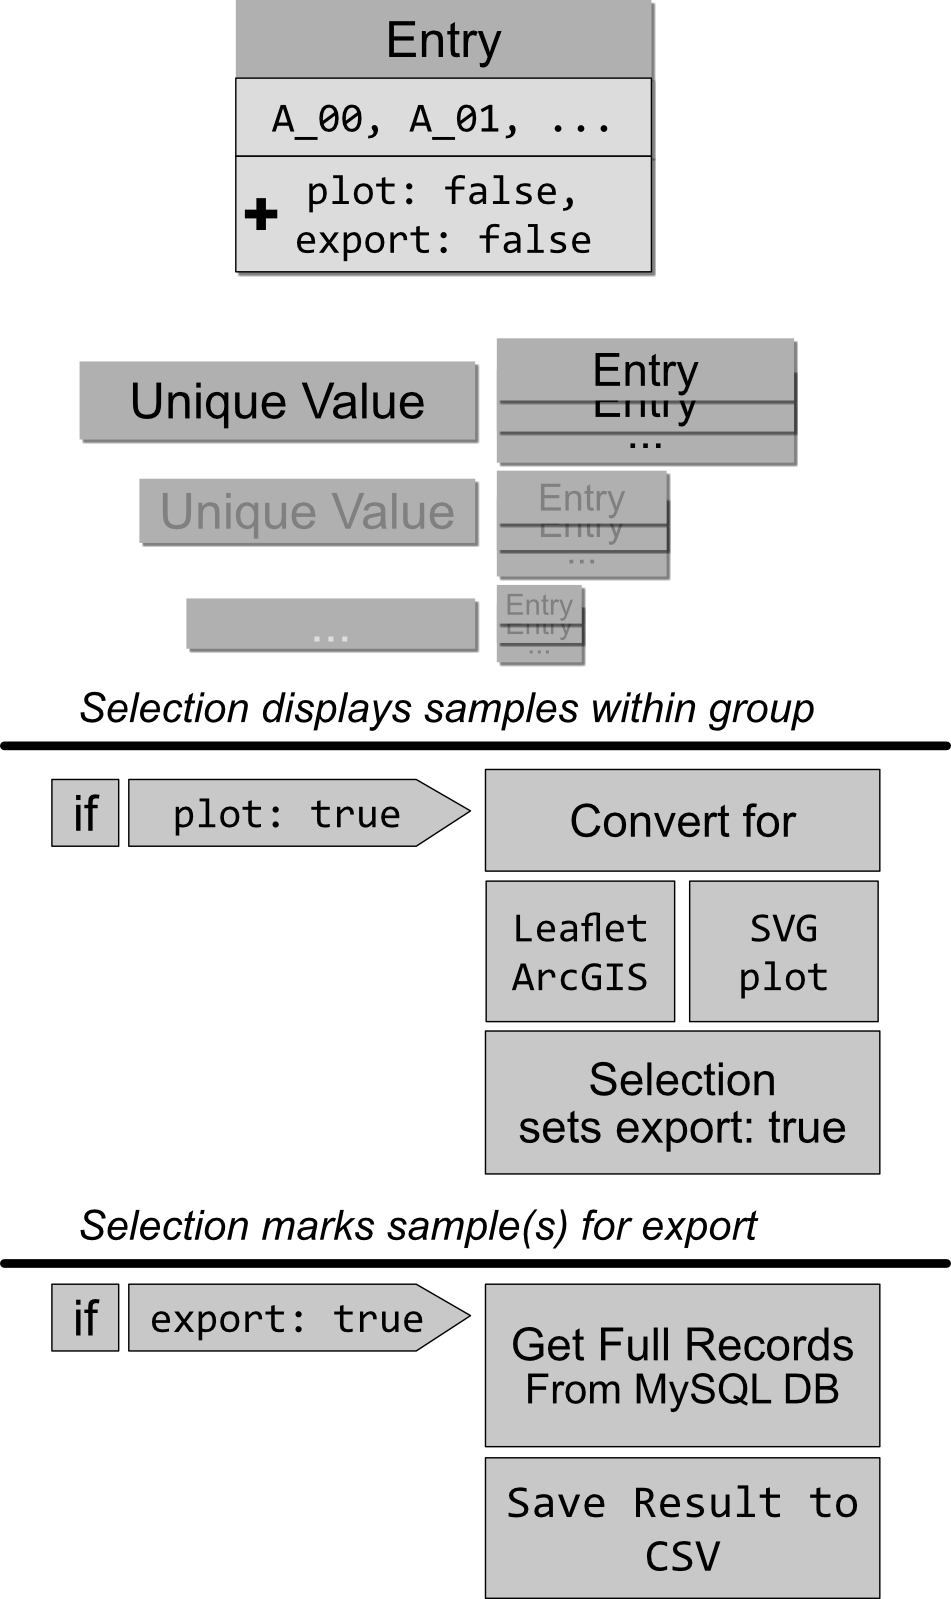
\includegraphics{figs/FigureTechnical.png}
	\caption{Data handling and processing within PALEO-SEAL.}
	\label{fig:3}
\end{figure}

\section{PALEO-SEAL applications}
In general, PALEO-SEAL can be used to visualize, query and download Holocene sea-level data related to a research project or a scientific paper. For example, we deployed PALEO-SEAL to showcase the data reviewed in the context of a research project on South-East Asia sea-level proxies by \citet{mann2019holocene}. The deployed interface is available at \href{https://warmcoasts.eu/paleo-seal/}{this link}. In general, the interface can be easily scaled up to thousands of points. Testing it with ca. 1000 records did not affect the query speed significantly. Papers similar to the available example are available from the areas listed in Table 1 of \citet{khan2019}. 

\section{Author contributions}
Jan Drechsel developed PALEO-SEAL, Nicole Khan worked on the database template, Alessio Rovere wrote the paper and supervised the tool development. 

\section{Data and code availability}
The code is available from GitHub at this link:\url{https://github.com/jDrechsel/PALEO-SEAL.git} or from Zenodo: link. PALEO-SEAL is released under the terms of the Apache License 2.0 (\url{http://www.apache.org/licenses/LICENSE-2.0}). An example of deployement is hosted at \url{https://warmcoasts.eu/paleo-seal/}. In case this deployement will become unavailable in the future, we included the hosted files in the GitHub folder \texttt{Working\_example}. 

\section{Acknowledgments}
The development of PALEO-SEAL was possible thanks to the financial support of the German Science Foundation (SEASCHANGE, DFG RO 5245/1-1), funded within the program 
``SPP 1889 Regional Sea Level Change and Society''. The interface builds on the data structure compiled by the HOLSEA project, funded by the International Union for Quaternary Research (INQUA) and on the activities of PALSEA, funded by INQUA and Past Global Changes (PAGES), which in turn received support from the Swiss Academy of Sciences and the Chinese Academy of Sciences.

%% Loading bibliography style file
%\bibliographystyle{model1-num-names}
\bibliographystyle{cas-model2-names}

% Loading bibliography database
\bibliography{cas-refs}

\end{document}

